\section{Results and discussion}
\label{sec:eval:resultsdiscussion}

% ----------------------- paths to graphics ------------------------

\graphicspath{{6_evaluation/images/}}

% ----------------------- contents from here ------------------------
% 

This section is structured as follows: we present and analyse the results obtained with Configuration A (iterative greedy) in \ref{subsec:eval:results:vectorwise}, \ref{subsec:eval:results:estimator} and \ref{subsec:eval:results:analysis} and the results obtained with Configuration B (recursive exhaustive)---plus comparison between the two---in \ref{subsec:eval:results:recursiveexhaustive}.

\subsection{VectorWise baseline results}
\label{subsec:eval:results:vectorwise}

We evaluated the \textit{whitebox compression} model against the \nameref{subsec:eval:methodology:vectorwise} according to the methodology (\ref{subsec:eval:methodology:vectorwise}). This section presents the results obtained with Configuration A (iterative greedy). Figure~\ref{fig:eval:results:vectorwise:total} shows the compression ratios---\(ratio_{blackbox}\), \(ratio_{whitebox}\)---and the 3 sizes they were derived from---\(size_{uncompressed}\), \(size_{blackbox}\), \(size_{whitebox}\)---for each table. The tables are sorted in descending order by \(ratio_{whitebox}\). In this figure we made the comparison for the full tables, including all logical columns, even though only a part of them are in the scope of \textit{whitebox compression}.

\begin{figure}[h]
  \centering
   \makebox[\textwidth][c]{
    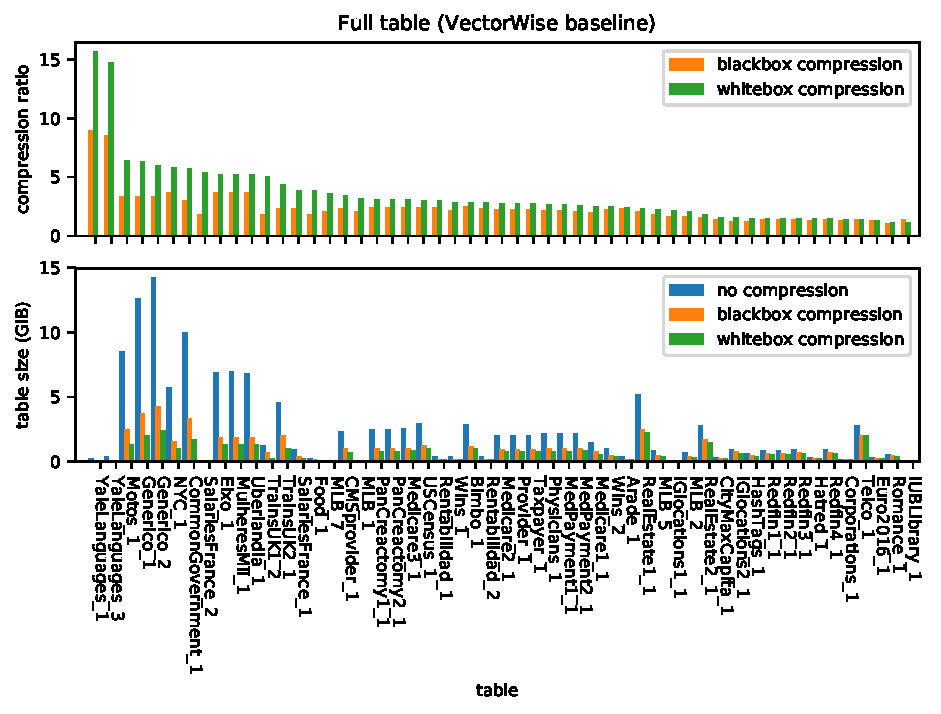
\includegraphics[width={1.1\linewidth}]{6_evaluation/images/vw_total.pdf}
    }
  \caption{Full table comparison (VectorWise baseline)}
  \label{fig:eval:results:vectorwise:total}
\end{figure}

The total size of the uncompressed tables is 131GB. The overall compression ratios are:  \(ratio_{blackbox} = 2.58\) and \(ratio_{whitebox} = 3.58\). \textit{Whitebox compression} has an overall ratio of 1.38 against blackbox compression. In the first chart we can observe that for one third of the tables \(ratio_{whitebox}\) is significantly higher than \(ratio_{blackbox}\). The rest of the tables have similar compression ratios. 
An important observation is that, even though \textit{whitebox compression} only brings a significant improvement to a small part of the tables, it is never worse than blackbox compression. The only exception is the last table, where \(ratio_{blackbox} = 1.38\) and \(ratio_{whitebox} = 1.11\). However, this table is extremely small in uncompressed format: 508KB. Such small data already fits in the CPU cache and does not require compression at all. We can further notice that most of the tables with high \(ratio_{blackbox}\) have even higher \(ratio_{whitebox}\) and those with the lowest \(ratio_{blackbox}\) have the lowest \(ratio_{whitebox}\). A possible explanation for this phenomenon is that \textit{whitebox compression} compresses the same columns as VectorWise---those with high repetition factors and redundancy---but manages to exploit these opportunities more efficiently and respectively, has a small improvement when there are no opportunities. From the second chart we can make the observation that the majority of the large tables tend to have higher compression ratios than most of the small tables, with some exceptions. This is particularly true for \textit{whitebox compression}, but also for blackbox, since the two are also somewhat correlated.

These results include all the logical columns, even tough some of them were not represented through \textit{whitebox compression}. Our compression model does not incur any overhead on these columns and therefore we can exclude them from the evaluation with the purpose of measuring the improvement more accurately. Figure~\ref{fig:eval:results:vectorwise:used} shows the same charts but only includes the columns represented through \textit{whitebox compression}. Measuring these results required column-level analysis. For this reason, we excluded the tables for which we couldn't match the columns with VectorWise's data files (because of multiple columns stored in the same file). Tables are sorted by the new \(ratio_{whitebox}\).

\begin{figure}[h]
  \centering
   \makebox[\textwidth][c]{
    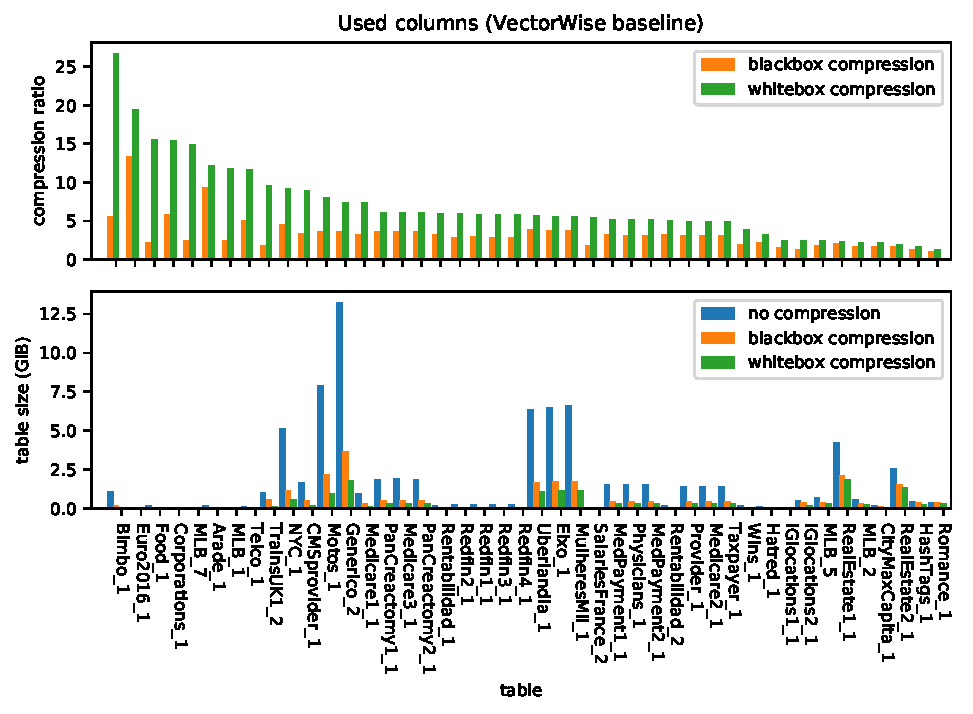
\includegraphics[width={1.1\linewidth}]{6_evaluation/images/vw_used.pdf}
    }
  \caption{Used columns comparison (VectorWise baseline)}
  \label{fig:eval:results:vectorwise:used}
\end{figure}

The results are as expected: the average compression ratio increased and \textit{whitebox compression} brings a significant improvement for the majority of the tables. Table~\ref{tab:eval:results:vectorwise:totalvsused} shows an overall comparison between the full table results and the used columns results.

\begin{table}[!h]
\centering
\begin{tabular}{c|cccc}
             & \begin{tabular}[c]{@{}c@{}}\(size_{uncompressed}\)\\ (GB)\end{tabular} & \(ratio_{blackbox}\) & \(ratio_{whitebox}\) & \(\frac{ratio_{blackbox}}{ratio_{whitebox}}\) \\ \hline
Full table   & 131                                                                    & 2.58                 & 3.58                 & 1.38                                          \\
Used columns & 77                                                                     & 3.16                 & 5.16                 & 1.63                                         
\end{tabular}
\caption{Full table vs. used columns (VectorWise baseline)}
\label{tab:eval:results:vectorwise:totalvsused}
\end{table}

Only 68\% of the total size of the data was represented through \textit{whitebox compression}. The increase of \(ratio_{blackbox}\) shows that columns used by \textit{whitebox compression} are also good candidates for  blackbox compression. However, \(ratio_{whitebox}\) increased more than \(ratio_{blackbox}\), indicating that \textit{whitebox compression} created opportunities for more compact representation.

The difference between the used columns evaluation and the full table evaluation is determined by the lack of opportunities for \textit{whitebox compression} in part of the data. For a better understanding, imagine that we want to compress two columns \(c_{a}\) and \(c_{b}\) of equal size \(s\). \(c_{a}\) presents no compression opportunities (\(ratio_{a} = 1\)) and \(c_{b}\) has \(ratio_{b} = 10\). Even though half of the data is highly compressible, the total ratio of the two columns is much lower: \(ratio_{total} = \frac{2 \times s}{s + 0.1 \times s} = 1.81\).

The conclusion that we can draw so far is that \textit{whitebox compression} achieves high compression ratios on the columns that it represents through the expression trees and is never worse than blackbox compression alone. Additionally, the columns that do not present compression opportunities are not affected and the underlying database system operates normally on them.


% ------------ estimator model ------------ %

\subsection{Estimator model baseline results}
\label{subsec:eval:results:estimator}

We conducted an additional evaluation of the \textit{whitebox compression} model, this time against the \nameref{subsec:eval:methodology:estimator}, with the purpose of measuring the compression capabilities of a stand-alone \textit{whitebox} system. The VectorWise blackbox compression schemes are replaced by the lightweight compression estimators defined in \ref{sub:estimators}. We followed the methodology described in \ref{subsec:eval:methodology:estimator}. This section presents the results obtained with Configuration A (iterative greedy). Figure~\ref{fig:eval:results:estimator:used} shows the compression ratios and table sizes, considering only the columns represented through \textit{whitebox compression}.

\begin{figure}[h]
  \centering
   \makebox[\textwidth][c]{
    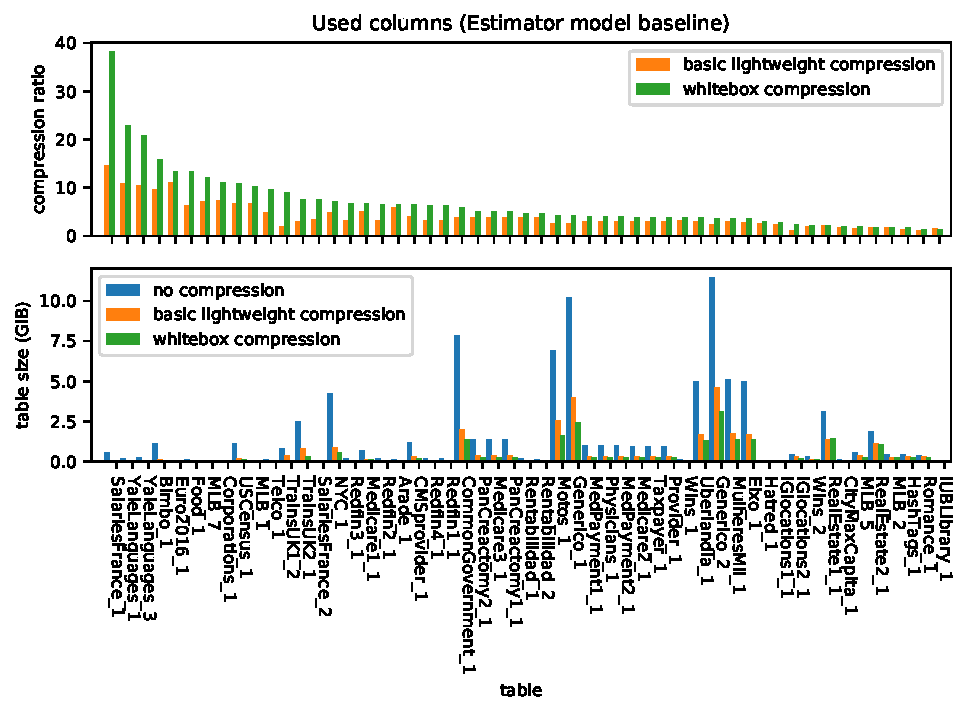
\includegraphics[width={1.1\linewidth}]{6_evaluation/images/estimator_used.pdf}
    }
  \caption{Used columns comparison (Estimator model baseline)}
  \label{fig:eval:results:estimator:used}
\end{figure}

The overall results are similar to the \nameref{subsec:eval:methodology:vectorwise}: \textit{whitebox compression} is effective for part of the tables (around 40\% of them in this case) and for the rest of them it gives similar compression ratios with the basic lightweight schemes. Similarly, the compression ratios are correlated: \(ratio_{whitebox}\) is higher respectively lower where \(ratio_{lightweight}\) is higher respectively lower. The same observation, that \textit{whitebox compression} is never worse than the basic lightweight compression schemes alone, is also true for the estimator baseline, with the same exception: the last table. Table~\ref{tab:eval:results:estimatorvsvectorwise} shows an overall comparison between the 2 baselines.

\begin{table}[!h]
\centering
\begin{tabular}{c|cccc}
                & \begin{tabular}[c]{@{}c@{}}\(size_{uncompressed}\)\\ (GB)\end{tabular} & \(ratio_{blackbox}\) & \(ratio_{whitebox}\) & \(\frac{ratio_{blackbox}}{ratio_{whitebox}}\) \\ \hline
VectorWise      & 77                                                                     & 3.16                 & 5.16                 & 1.63                                          \\
Estimator model & 83                                                                     & 2.87                 & 4.04                 & 1.40                                         
\end{tabular}
\caption{VectorWise baseline vs. estimator model baseline (used columns)}
\label{tab:eval:results:estimatorvsvectorwise}
\end{table}

The total size of the used columns is 7\% higher and the compression ratios decreased with 9\% for the lightweight schemes and 21\% for \textit{whitebox compression}. The improvement of \textit{whitebox compression} is also a bit lower (14\% decrease). The \nameref{subsec:eval:methodology:estimator} seems to reduce the impact of both compression systems and in particular the effect of our model. However, the objective of \textit{whitebox compression}---to create compression opportunities for more compact data representation---is still met, since it brings an increase in compression ratio from 2.87 to 4.04.

Figure~\ref{fig:eval:results:estimatorvsvw} creates a better picture of the differences between the 2 baselines---a comparison of the table sizes for the three metrics in the methodology: \(size_{uncompressed}\), \(size_{lightweight}\)/\(size_{blackbox}\) and \(size_{whitebox}\).

\begin{figure}[h]
  \centering
   \makebox[\textwidth][c]{
    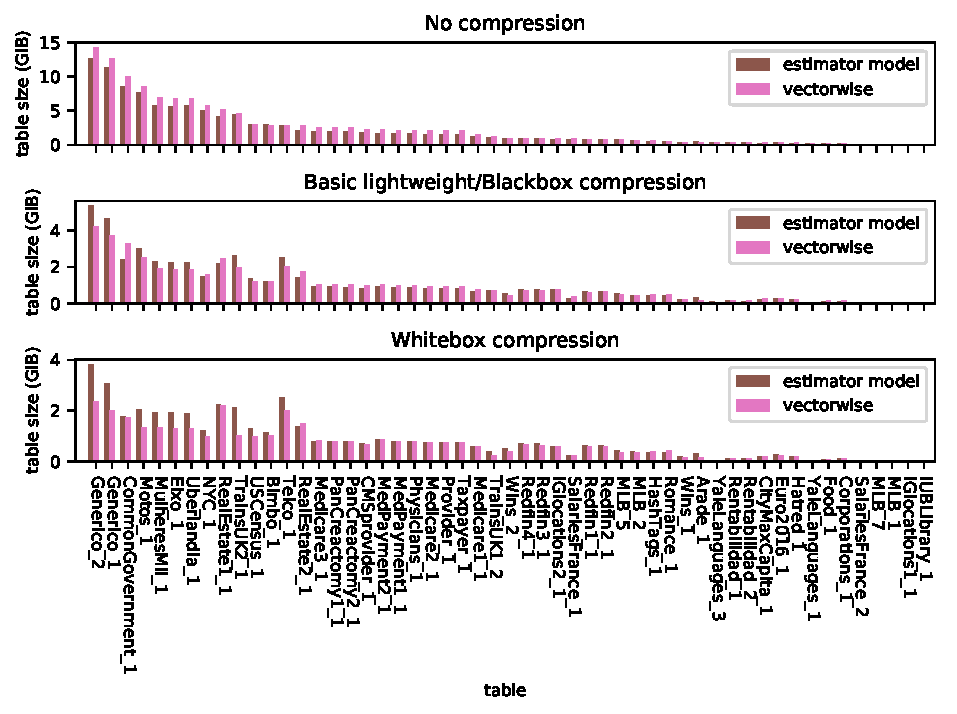
\includegraphics[width={1.1\linewidth}]{6_evaluation/images/estimator_vs_vw_combined.pdf}
    }
  \caption{Baseline comparison (full table): Estimator model vs. Vectorwise}
  \label{fig:eval:results:estimatorvsvw}
\end{figure}

In the first chart we can see that the estimated uncompressed size of the data is a bit smaller than the VectorWise size for most tables. This result is not unexpected, since the storage layer of a real system is more complex and might add additional overhead compared to the theoretical estimation that we made. Moreover, the exact representation of each data type might differ from the one that we used. The second chart shows how VectorWise's blackbox compression schemes perform better than the (estimated) lightweight compression methods for some tables. This is not a surprising result, since our lightweight compression schemes are not optimized and the exception handling mechanism is different. A somewhat unexpected result can be observed in the third chart: VectorWise is even better at compressing the whitebox representation of the data than the estimator model for some tables. A possible explanation might be that the number, type and size of the physical columns differ, as \textit{whitebox compression} creates many nullable columns because of the exception handling mechanism, while VectorWise stores exceptions together with the compressed data, in blocks with custom format. Moreover, the compression metadata differs and its size is computed in a different way. An additional notable observation is that the difference between VectorWise and the estimator model is usually higher where the size of the data is larger, while for smaller tables the two models give closer results.

The overall conclusion that we can draw from this experiment is that, even though the two models give somewhat different results, \textit{whitebox compression} still brings a significant improvement over the existing lightweight compression methods. The main reason for the lower compression ratios of the \nameref{subsec:eval:methodology:estimator} is the different---and unoptimized---compression schemes. A more thorough experiment and analysis needs to be performed in order to properly evaluate the performance of a stand-alone \textit{whitebox} system in practice---we leave this for future work. Even so, we showed that \textit{whitebox compression} can be used to enhance existing systems---like VectorWise---as an intermediate layer before the optimized compression methods.


% ------------ analysis ------------ %

\subsection{Results analysis}
\label{subsec:eval:results:analysis}

To better understand the impact of \textit{whitebox compression} and how it represents the data, we performed an analysis of the physical data size components and the expression trees. We conducted this analysis on the results obtained with the VectorWise methodology (\ref{subsec:eval:methodology:vectorwise}). This section presents the results obtained with Configuration A (iterative greedy).

\begin{figure}[h]
  \centering
  \makebox[\textwidth][c]{
  \begin{subfigure}[t]{0.6\linewidth}
    \centering
    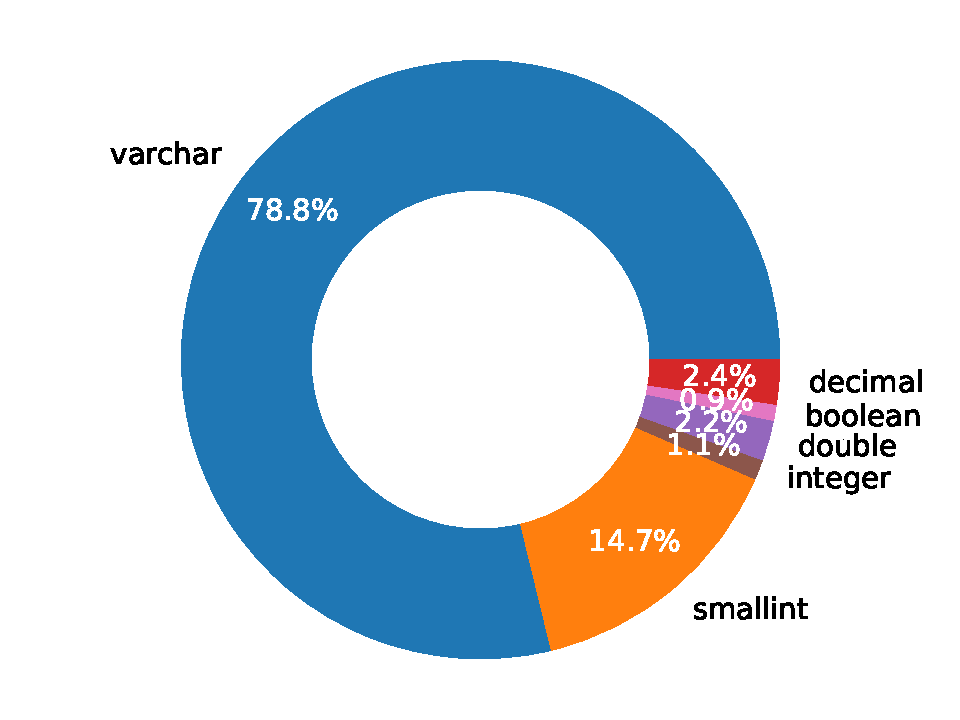
\includegraphics[width=1\linewidth]{6_evaluation/images/used_datatypes.pdf}
    \caption[b]{Logical columns (used)}
    \label{fig:eval:results:useddatatypes}
  \end{subfigure}
%   \hspace{1em}
  \begin{subfigure}[t]{0.6\linewidth}
    \centering
    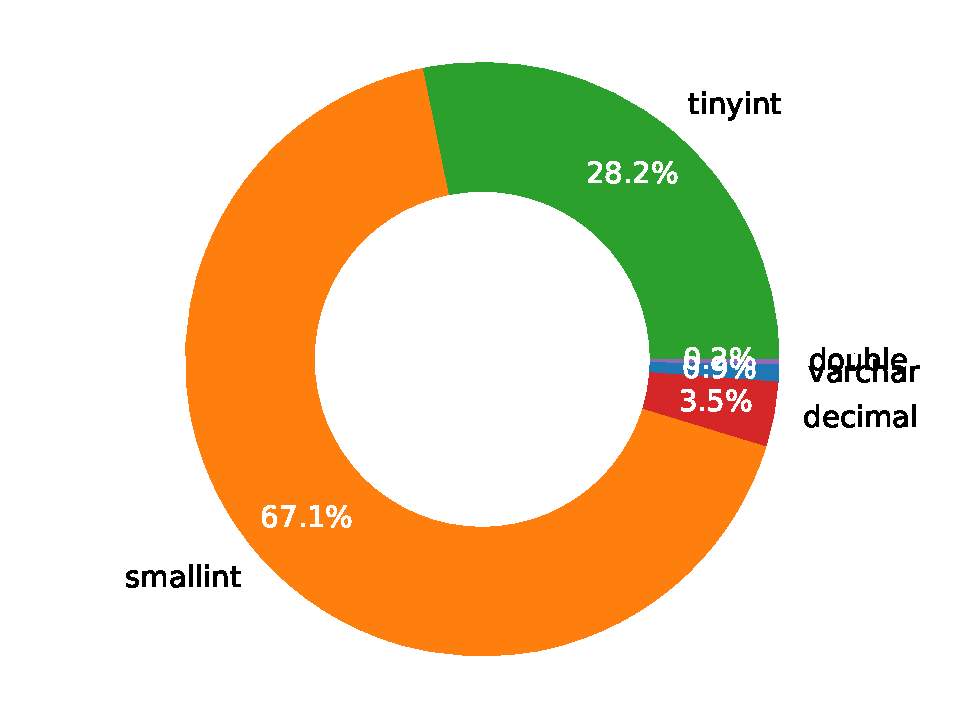
\includegraphics[width=1\linewidth]{6_evaluation/images/out_datatypes.pdf}
    \caption[b]{Physical columns}
    \label{fig:eval:results:outdatatypes}
  \end{subfigure}
  }
  \caption{Column datatype distribution}
  \label{fig:eval:results:columndatatypes}
\end{figure}

Figure~\ref{fig:eval:results:useddatatypes} shows the distribution of datatypes across the logical columns represented through \textit{whitebox compression}. The majority of columns are \verb|VARCHAR|, since our system leverages the opportunities present in strings. The rest of the columns are numeric and boolean and are all constant columns, since the \nameref{subsec:pd:constant} pattern detector is the only one that works on other datatypes than strings. Figure~\ref{fig:eval:results:outdatatypes} shows the distribution of datatypes across the physical columns resulted after the \textit{whitebox} representation (excluding exception columns). With the exception of 1\% \verb|VARCHAR| columns, all the other are numeric. They resulted from \nameref{subsec:pd:numericstrings} and \nameref{subsec:pd:dict} representations (observation: dictionary ids are stored in SQL numeric datatypes so that they can be loaded into VectorWise; however, the main purpose of \nameref{subsec:pd:dict} expression nodes is to serve as an intermediate representation layer before \nameref{subsec:pd:columncorrelation}). The only pattern detector that outputs \verb|VARCHAR| columns is \nameref{subsec:pd:charsetsplit}. The other 2 pattern detectors---\nameref{subsec:pd:constant} and \nameref{subsec:pd:columncorrelation}---do not output any physical columns. Instead, they reduce the number of columns by consuming them and only storing metadata.

Table~\ref{tab:eval:results:analysis2} shows the impact of \textit{whitebox compression} through an analysis of the logical and physical columns in terms of numbers and sizes. 

\begin{table}[!h]
\centering
\begin{tabular}{cc|c|cc}
                         &           & Logical columns & \multicolumn{2}{c}{Physical columns} \\
                         &           & Used columns    & Data columns   & Exception columns   \\ \hline
\multirow{2}{*}{Average} & Count     & 26              & 8              & 46                  \\
                         & Size (MB) & 1.45GB          & 85MB           & 262MB               \\ \hline
\multirow{2}{*}{Total}   & Count     & 1406            & 462            & 2479                \\
                         & Size      & 77.2GB          & 3.7GB          & 11.3GB             
\end{tabular}
\caption{Logical vs. physical columns}
\label{tab:eval:results:analysis1}
\end{table}

On the average table, there are 26---out of 67 (38\%)---logical columns used in the \textit{whitebox} representation. They are represented through only 8 physical columns containing compressed data and an additional 46 exception columns. The number of data columns is reduced because of the expression nodes that consume columns: \nameref{subsec:pd:constant} and \nameref{subsec:pd:columncorrelation}. The number of exception columns is very high due to our option to keep an exception column for each expression node in the tree and to allow recursive compression of exception columns. However, these columns are very sparse and contain mostly null values---which are effectively stored by the underlying database system through a bitmap. In terms of size, the average of 1.45GB of input data is represented through only 85MB of compressed data and 262MB of exceptions. Therefore, 1.19GB of the data (non-exceptions: 1.45GB - 262MB) is represented through 85MB of compressed data---plus the size of the metadata, which is insignificant (see Figure~\ref{fig:eval:results:outsizedistribution}). These results show the high degree of redundancy present in real data---and that we can squeeze this redundancy out of the data if we have a proper exception handling mechanism.
Table~\ref{tab:eval:results:analysis1} also shows the same analysis for the overall results---total of all tables---instead of the average.

\begin{figure}[h]
\centering
\makebox[\textwidth][c]{
\begin{minipage}{0.55\textwidth}
  \centering
  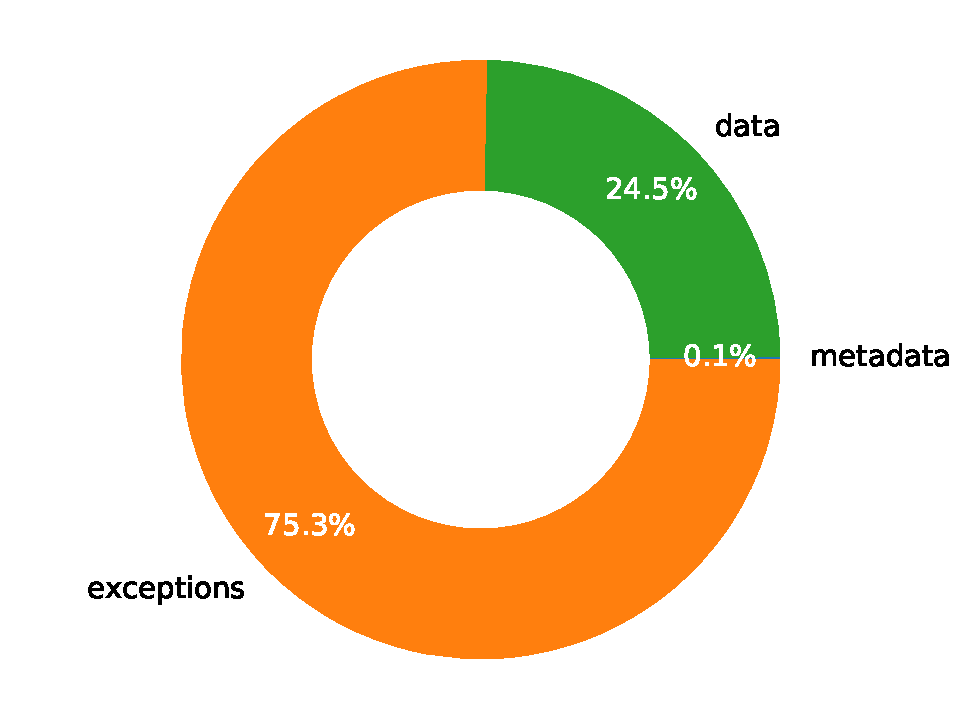
\includegraphics[width={1.0\linewidth}]{6_evaluation/images/out_size_distribution.pdf}
  \caption{Physical size distribution}
  \label{fig:eval:results:outsizedistribution}
\end{minipage}
% \hspace{1em}
\begin{minipage}{0.55\textwidth}
  \centering
  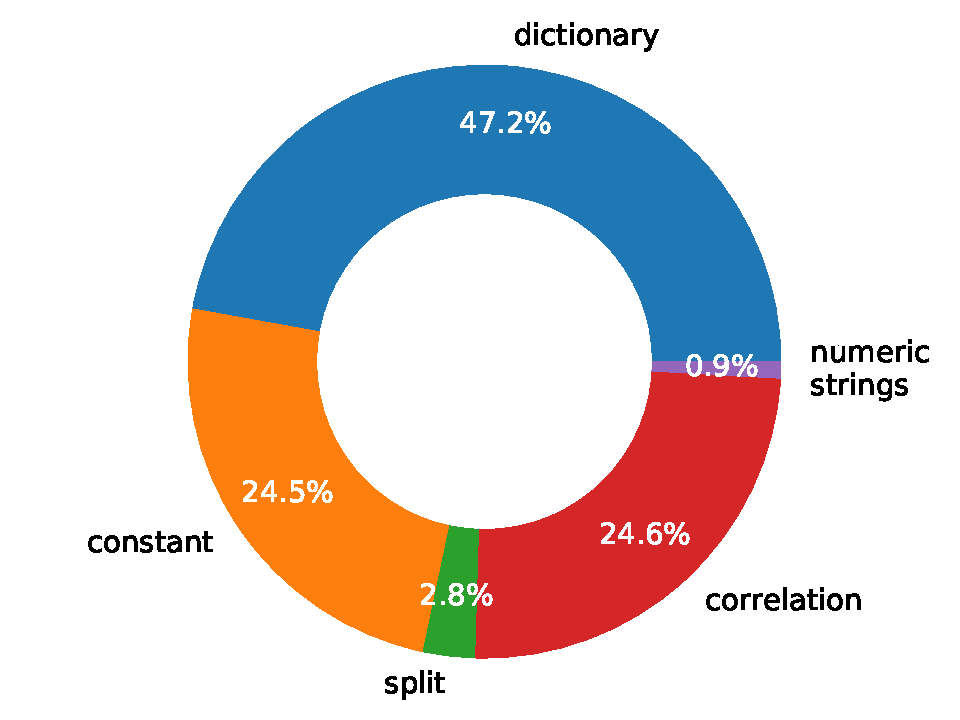
\includegraphics[width={1.0\linewidth}]{6_evaluation/images/expr_n_types.pdf}
  \caption{Expression node types distribution}
  \label{fig:eval:results:exprntypedistribution}
\end{minipage}
}
\end{figure}

Figure~\ref{fig:eval:results:outsizedistribution} shows a better picture of the physical data size distribution and the components that make it up. The exceptions sum up to 75.3\% while the compressed data represents 24.5\% of the total physical data size. The compression metadata (e.g. dictionaries, correlation maps, etc.) is insignificant, since we used a single compression tree for the entire table. The alternative---handling blocks of data separately---would allow a more fined grained representation with possibly simpler compression trees, at the expense of increasing the total metadata size. 

We also computed the exception ratio in terms of numbers instead of size (i.e. how \textit{many} exceptions there are) as follows: \(\frac{count_{exception}}{count_{input}}\), where \(count_{exception}\) is the total number of values on all leaf exception columns (i.e. physical columns, not further represented through other operators) and \(count_{input}\) is the total number of values on the corresponding parent columns from which the exceptions originated, which can be either inner or logical columns. We obtained an overall exception ratio of 0.16. Given the fact that exceptions make most of the physical size, reducing the exception ratio may be a way of achieving higher compression ratios. A more thorough analysis of these results, with a focus on exceptions, should be performed in order investigate ways of reducing the exception ratio---we leave it for future work.

For the rest of our analysis we focused our attention on the expression trees. Recall that the so called expression tree is actually a directed acyclic graph (DAG) with multiple root nodes and connected components (\ref{ch:exprlang}~\nameref{ch:exprlang}). Each connected component represents a subset of the logical columns as a function of physical columns. Table~\ref{tab:eval:results:analysis2} shows the characteristics of the average expression tree.

\begin{table}[!h]
\centering
\begin{tabular}{c|cccc}
Connected components   & Expression nodes & Depth & Logical columns & Physical columns \\
(on average per table) & \multicolumn{4}{c}{(on average per connected component)}  \\ \hline
12.5                   & 3.3              & 1.4   & 1.7           & 0.8           
\end{tabular}
\caption{Expression tree statistics}
\label{tab:eval:results:analysis2}
\end{table}


There are 12.5 connected components, with an average of 3.3 expression nodes and a depth of 1.4 levels. This shows that expression trees are not very complex and relatively fast to evaluate. A connected component represents on average 1.7 logical columns as a function of 0.8 physical columns (excluding exception columns)---the 0.8 value is due to the expression nodes that do not output any physical columns: \nameref{subsec:pd:constant} and \nameref{subsec:pd:columncorrelation}. Here we see again the capacity of \textit{whitebox compression} to reduce the number of columns by storing metadata instead.
% Moreover, the dependencies between columns are not that high, given the small number of logical and physical columns.
% However, these results are showing the average. There are many complex connected components and even more simple ones with only one expression node.

% TODO-1: create histograms with the metrics in Table~\ref{tab:eval:results:analysis2}.

Finally, Figure~\ref{fig:eval:results:exprntypedistribution} shows the distribution of the expression node types in the average expression tree. In this analysis we considered both internal and leaf nodes. We notice that the majority is composed of \nameref{subsec:pd:constant}, \nameref{subsec:pd:dict} and \nameref{subsec:pd:columncorrelation}, while only a small percentage are \nameref{subsec:pd:charsetsplit} and \nameref{subsec:pd:numericstrings}. This is due to the high \nameref{subsec:pd:dict} compression potential of the data and to the high correlation between columns---high redundancy in other words. The split operators create opportunities for compressing subcolumns and thus, for every \nameref{subsec:pd:charsetsplit} node there are many \nameref{subsec:pd:constant}, \nameref{subsec:pd:dict} and \nameref{subsec:pd:columncorrelation} nodes. Also note that all \nameref{subsec:pd:columncorrelation} nodes take as input---and consume---\nameref{subsec:pd:dict} expression nodes. Therefore, the majority of the \nameref{subsec:pd:dict} nodes are internal nodes of the expression tree. An additional reason for this distribution of expression nodes is the priority configuration that we used for this experiment---recall that \nameref{subsec:pd:constant} and \nameref{subsec:pd:dict} have the highest priority (\ref{sec:eval:expsetup}~\nameref{sec:eval:expsetup}). We also experimented with other configurations of the \nameref{subsubsec:ps:priority} which resulted in more even distributions of the expression node types, but decided to show the results of this configuration because they were better. Moreover, we will see in the next section that this choice of expression node types is also optimal with respect to our cost model (\ref{sub:estimators}), since the \nameref{sub:learning:recursiveexhaustive} algorithm produced a similar distribution, while trying to minimize the physical data size.

% From our experiments we concluded that data can be represented and compressed in many ways. However, the learning algorithm needs to choose a single data representation, ideally the one that gives the smallest physical size.

The take-away message from this analysis is that we can represent many logical columns---mostly \verb|VARCHAR|---as functions of fewer physical columns---mostly numeric---at the expense of many exception columns---mostly nulls---and achieve high compression ratios---all of this automatically learned.

% ------------ analysis ------------ %

\subsection{Recursive exhaustive learning results}
\label{subsec:eval:results:recursiveexhaustive}

We repeated the same experiments presented so far, this time with Configuration B (recursive exhaustive). This section presents an analysis of the results in comparison to the ones obtained with Configuration A (iterative greedy). As expected, the non-greedy, cost model-based approach brought an improvement in terms of compression ratio.

\begin{table}[h]
\centering
% \small
\makebox[\textwidth][c]{
\begin{tabular}{cl|cccc}
                                                                        &                      & \begin{tabular}[c]{@{}c@{}}\(size_{uncompressed}\)\\ (GB)\end{tabular} & \(ratio_{blackbox}\)  & \(ratio_{whitebox}\) & \(\frac{ratio_{blackbox}}{ratio_{whitebox}}\) \\ \hline
\multirow{2}{*}{\begin{tabular}[c]{@{}c@{}}Full\\ table\end{tabular}}   & Iterative greedy     & \multirow{2}{*}{131}                                                   & \multirow{2}{*}{2.58} & 3.58                 & 1.38                                          \\ \cline{2-2} \cline{5-6} 
                                                                        & Recursive exhaustive &                                                                        &                       & 3.69                 & 1.43                                          \\ \hline
\multirow{2}{*}{\begin{tabular}[c]{@{}c@{}}Used\\ columns\end{tabular}} & Iterative greedy     & 77                                                                     & 3.16                  & 5.16                 & 1.63                                          \\ \cline{2-6} 
                                                                        & Recursive exhaustive & 98                                                                     & 3.35                  & 6.45                 & 1.92                                         
\end{tabular}
}
\caption{Iterative greedy vs. Recursive exhaustive (VectorWise baseline)}
\label{tab:eval:results:recexh:vectorwise:totalvsused}
\end{table}


Table~\ref{tab:eval:results:recexh:vectorwise:totalvsused} shows the sizes and compression ratios obtained with the two configurations. For the full data, Configuration B gave a slightly higher compression ratio, leading to an overall improvement of 1.43 over VectorWise. The two algorithms resulted in different compression trees and thus the columns represented through \textit{whitebox compression} are not the same. Because of this, \(size_{uncompressed}\) and \(ratio_{blackbox}\) differ for the used columns: the recursive exhaustive algorithm selected a larger subset of the data (74\% of the total size), which is also compressed slightly better by VectorWise. \textit{Whitebox compression} achieves a significantly higher compression ratio of 6.45 on the used columns---an improvement of \(1.92\times\) over the existing blackbox methods.

\begin{table}[h]
\centering
\begin{tabular}{cc|c|cc}
                         &           & Logical columns & \multicolumn{2}{c}{Physical columns} \\
                         &           & Used columns    & Data columns   & Exception columns   \\ \hline
\multirow{2}{*}{Average} & Count     & 22              & 7              & 41                  \\
                         & Size (MB) & 1.96GB          & 56MB           & 256MB               \\ \hline
\multirow{2}{*}{Total}   & Count     & 1072            & 373            & 2046                \\
                         & Size      & 98.1GB          & 2.7GB          & 12.5GB             
\end{tabular}
\caption{Logical vs. physical columns (recursive exhaustive learning)}
\label{tab:eval:results:recexh:analysis1}
\end{table}

\begin{figure}[h]
  \centering
  \makebox[\textwidth][c]{
  \begin{subfigure}[t]{0.6\linewidth}
    \centering
    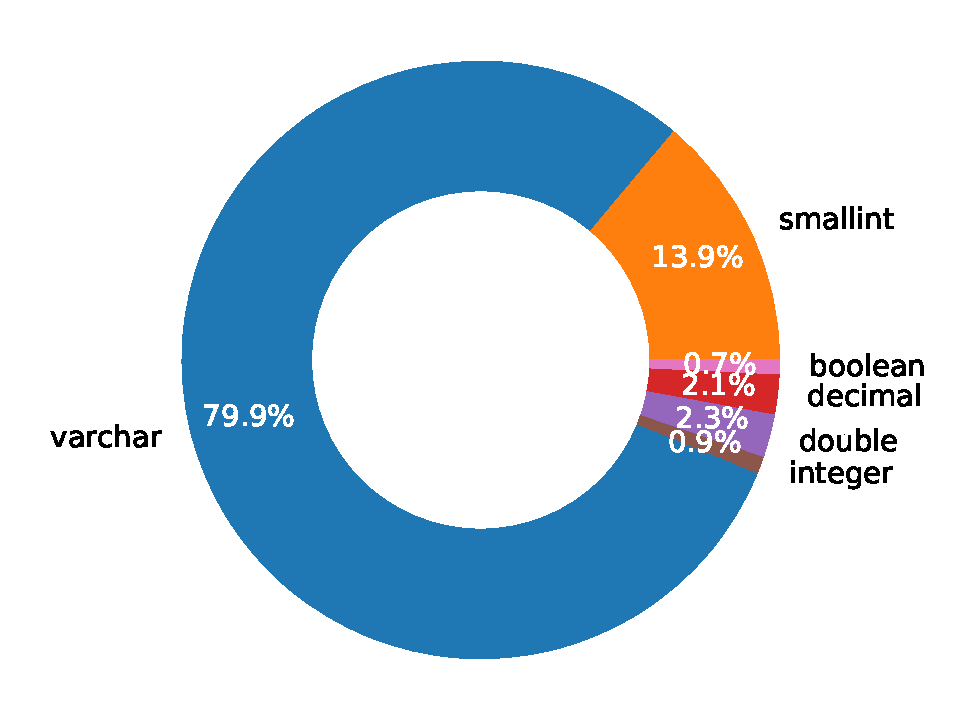
\includegraphics[width=1\linewidth]{6_evaluation/images/rec_exh/used_datatypes.pdf}
    \caption[b]{Logical columns (used)}
    \label{fig:eval:results:recexh:useddatatypes}
  \end{subfigure}
%   \hspace{1em}
  \begin{subfigure}[t]{0.6\linewidth}
    \centering
    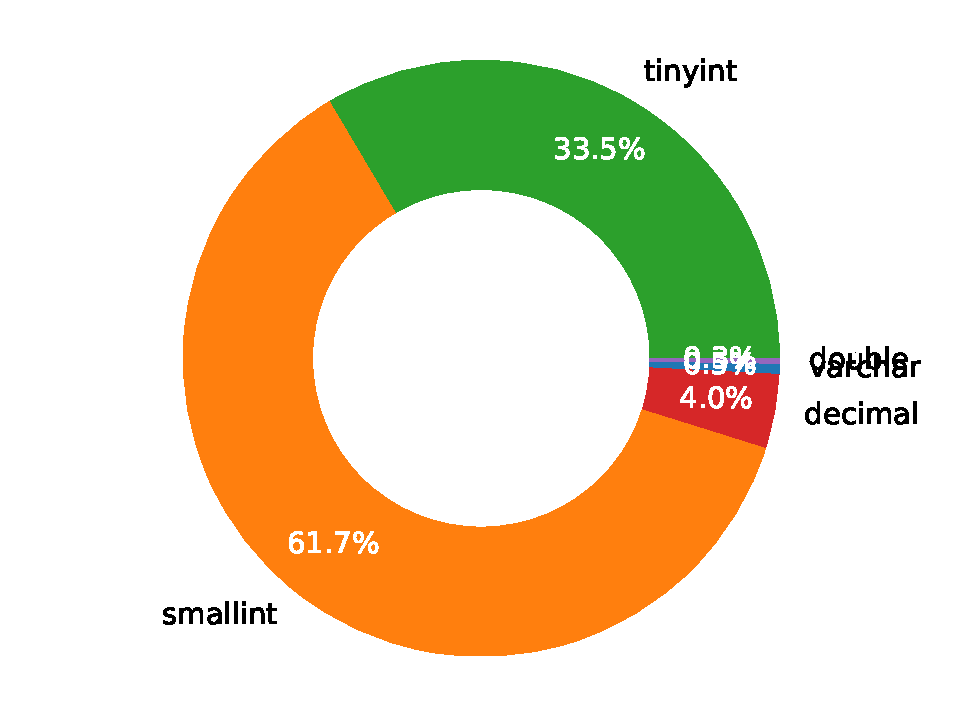
\includegraphics[width=1\linewidth]{6_evaluation/images/rec_exh/out_datatypes.pdf}
    \caption[b]{Physical columns}
    \label{fig:eval:results:recexh:outdatatypes}
  \end{subfigure}
  }
  \caption{Column datatype distribution (recursive exhaustive learning)}
  \label{fig:eval:results:recexh:columndatatypes}
\end{figure}

Table~\ref{tab:eval:results:recexh:analysis1} and Figure~\ref{fig:eval:results:recexh:columndatatypes} show a analysis of the logical and physical columns. Configuration B used less logical columns than Configuration A, but with a larger overall size. The distribution of datatypes across these columns is similar in both cases: \(\approx80\%\) \verb|VARCHAR| and \(\approx20\%\) other datatypes. In terms of physical columns, the compressed data columns are both fewer in numbers and smaller in size. The total number of exception columns is 17\% smaller but their total size is 9\% higher---in a similar trend with the logical columns. The datatype distribution across the physical columns is also similar: >99\% numeric, with an increase of the \verb|TINYINT| percentage at the expense of \verb|SMALLINT|. Figure~\ref{fig:eval:results:recexh:outsizedistribution} shows how the total physical size is split between compressed data, exceptions and metadata. Similarly to Configuration A, metadata is insignificant and exceptions make up most of the size. The exception ratio (in terms of numbers) is slightly smaller: 0.15 instead of 0.16.

\begin{figure}[h]
\centering
\makebox[\textwidth][c]{
\begin{minipage}{0.55\textwidth}
  \centering
  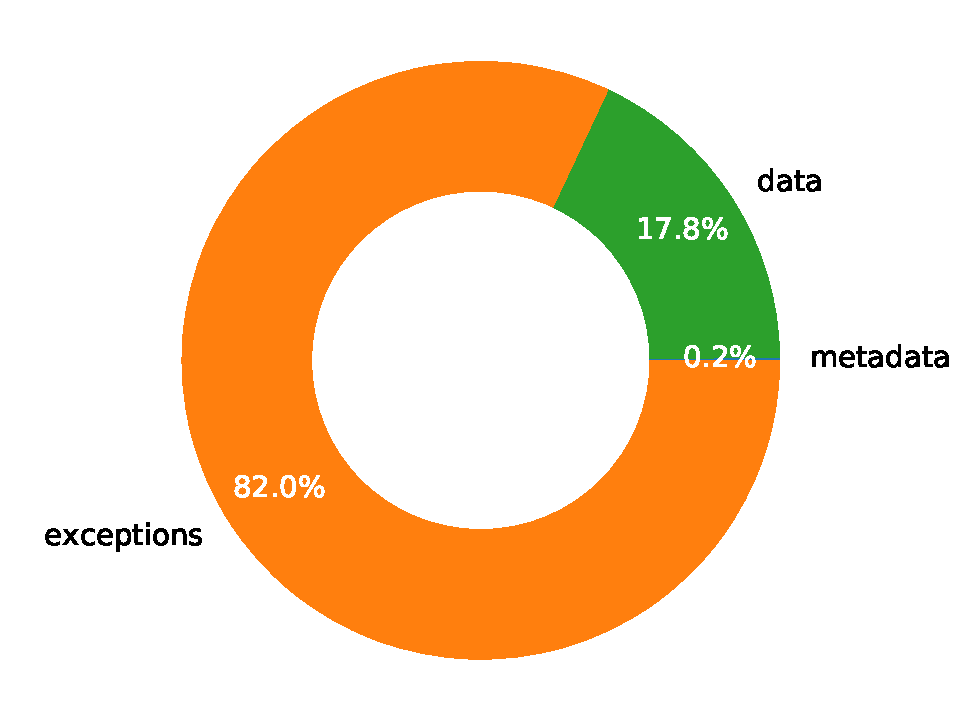
\includegraphics[width={1.0\linewidth}]{6_evaluation/images/rec_exh/out_size_distribution.pdf}
  \caption{Physical size distribution (recursive exhaustive learning)}
  \label{fig:eval:results:recexh:outsizedistribution}
\end{minipage}
% \hspace{1em}
\begin{minipage}{0.55\textwidth}
  \centering
  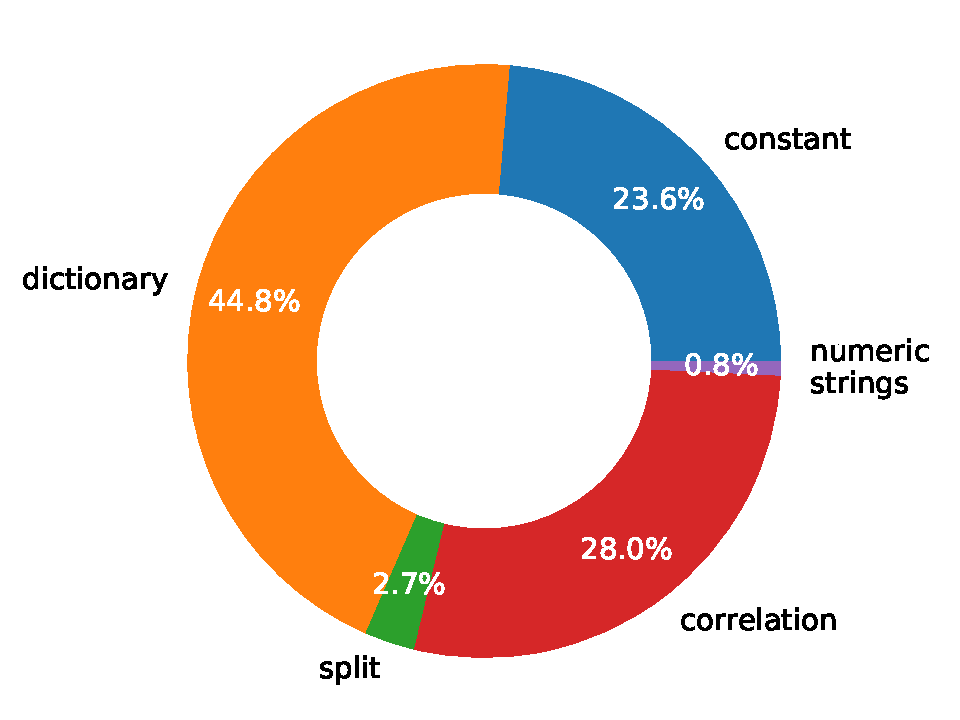
\includegraphics[width={1.0\linewidth}]{6_evaluation/images/rec_exh/expr_n_types.pdf}
  \caption{Expression node types distribution (recursive exhaustive learning)}
  \label{fig:eval:results:recexh:exprntypedistribution}
\end{minipage}
}
\end{figure}

\begin{table}[h]
\centering
\begin{tabular}{c|cccc}
Connected components   & Expression nodes & Depth & Logical columns & Physical columns \\
(on average per table) & \multicolumn{4}{c}{(on average per connected component)}  \\ \hline
11.5                   & 3.6              & 1.3   & 1.9           & 0.7           
\end{tabular}
\caption{Expression tree statistics (recursive exhaustive learning)}
\label{tab:eval:results:recexh:analysis2}
\end{table}


Figure~\ref{fig:eval:results:recexh:exprntypedistribution} and Table~\ref{tab:eval:results:recexh:analysis2} present the results of the expression tree analysis. The distribution of expression nodes is similar to the one given by Configuration A, with a slight increase of the \nameref{subsec:pd:columncorrelation} percentage and decrease of \nameref{subsec:pd:dict} and \nameref{subsec:pd:constant} percentages. Moreover, the expression trees are comparable in terms of structure (number of connected components, nodes, depth, logical and physical columns). These results confirm that the rules and heuristics used in the \nameref{sub:learning:iterative} algorithm and the configuration of the \nameref{subsubsec:ps:priority} are suitable choices, since the greedy algorithm is capable of exploiting compression opportunities in similar ways as the exhaustive algorithm does.

We have seen how Configuration B (recursive exhaustive) achieves higher compression ratios than Configuration A (iterative greedy) by using an exhaustive search based on the compression estimation cost model (\ref{sub:estimators}) instead of making greedy choices based on pattern selection heuristics (\ref{sub:learning:selectors}). This improvement comes at the cost of compression learning time. Our \verb|Python| implementation of the learning engine takes around 1 minute with Configuration A and around 5 minutes with Configuration B to learn the compression tree for a table, depending on the sample size, number and type of columns. Most of this time is spent by analysing the sample for each (sub)column with the pattern detectors and, in the case of Configuration B, by estimating the size of each (sub)column with the compression estimators. The execution time of the recursive exhaustive algorithm is limited by the maximum height threshold that we imposed on the expression tree. Adjusting this threshold might result in better compression ratios at the cost of longer learning times.

All in all, we defined and evaluated two different \textit{whitebox compression} learning algorithms which create compact representations of the data. Their execution times can be improved through more efficient implementations in lower level programming languages, but even so, they are practical, as compression learning happens during bulk loading of the data.

% TODO-2: new subsection about decompression implementation to validate input data reconstruction

\iffalse
reducing the exception ratio (e.g. through more granular subsets of values on the same columns represented differently -> smaller coverage\_min threshold) should increase the compression ratio, but will inevitably lead to a more complex learning process and complex expression trees. Another way of reducing exceptions without increasing the granularity/etc. is through more general pattern detectors that fit data better, but this may lead to less compact representation of the data and implicitly larger physical data and smaller compression ratios.
\fi

% ---------------------------------------------------------------------------
% ----------------------- end of thesis sub-document ------------------------
% ---------------------------------------------------------------------------